\chapter{Estrazione di Grafi Basati sul Contenuto}

\section{Pipeline di Elaborazione del Linguaggio Naturale sul Contenuto}

Il natural language processing {\`e} una branca dell'intelligenza artificiale che concerne l'elaborazione automatica del linguaggio naturale. Trattandosi di un processo particolarmente complesso a causa delle caratteristiche intrinseche di ambiguit{\`a} del linguaggio umano, tra cui sinonimia e polisemia, esso viene suddiviso in fasi diverse. Lo scopo {\`e} quello di determinare la funzione delle singole parole, che vengono suddivise in classi sintattiche (nomi, verbi, aggettivi e avverbi), in base alla loro funzione all'interno di una frase.

Lo Stanford NLP\footnote{Natural Language Processing} Group {\`e} uno dei gruppi di ricerca di maggiore importanza nel settore dell'elaborazione del linguaggio naturale ed offre validi strumenti per realizzare tale scopo. Attraverso le \href{https://github.com/stanfordnlp/CoreNLP}{API Java} del modulo software \href{https://stanfordnlp.github.io/CoreNLP/}{CoreNLP} {\`e} possibile analizzare il dataset corpus per poter distinguerne le parole (tokenization), lemmatizzarle, nonch{\`e} ridurle alla loro forma canonica, e determinarne la funzione (PoS\footnote{Part of Speech} tagging) all'interno della frase. {\`E} cos{\`i} possibile classificarle nelle categorie sintattiche di nostro interesse che includono:

\paragraph{Nomi}

\begin{enumerate}[label=(\roman*)]
  
\item \textit{NN}: singolare;
\item \textit{NNP}: proprio singolare;
\item \textit{NNS}: plurale;
\item \textit{NNPS}: proprio plurale.

\end{enumerate}

\paragraph{Verbi}

\begin{enumerate}[label=(\roman*)]
  
\item \textit{VB}: forma base;
\item \textit{VBD}: passato;
\item \textit{VBG}: gerundio o participio presente;
\item \textit{VBN}: participio passato;
\item \textit{VBP}: presente singolare (esclusa terza persona singolare);
\item \textit{VBZ}: presente, terza persona singolare.

\end{enumerate}

\begin{figure}\centering
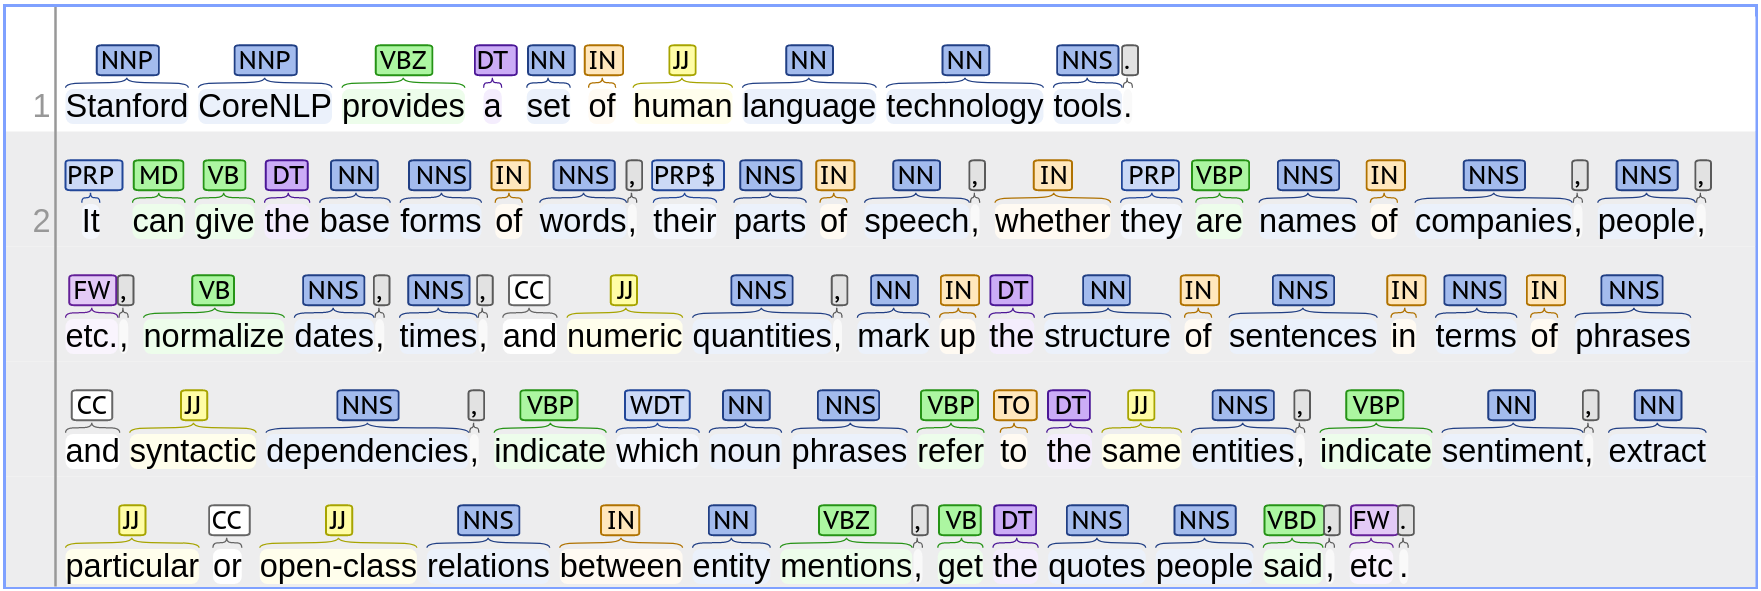
\includegraphics[scale=0.20]{img/pos}
\caption{Esempio di part-of-speech tagging.}
\end{figure}

\section{Identificazione di Archi Basati su Similarit{\`a}}
Il risultato della fase di NLP, costituita dai verbi e dai nomi lemmatizzati, si presta ad essere utilizzato per l'estrazione di caratteristiche linguistiche.

\subsection{Archi Basati su Similarit{\`a} Lessicale}
La similarit{\`a} lessicale tra i messaggi {\`e} stata calcolata grazie ad una versione modificata del Lexical Match Algorithm (LMA) \cite{hic} che considera i messaggi che si presuppone possano essere simili. Il LMA integra il Vector Space Model (VSM), nonch{\`e} uno dei pi{\`u} popolari metodi usati per identificare somiglianze lessicali. La formula del LMA per calcolare la similarit{\`a} lessicale produce un valore compreso tra 0 e 1 e pu{\`o} essere formalizzata come segue:

\begin{equation}
\sum_{i=0}^{LenX} {\sum_{j=0}^{LenY}}_{if POS(X_{i}) = POS(Y_{j})} \frac{TF_{X_{i}} + TF_{Y_{j}}}{DF_{X_{i}} + DF_{Y_{j}}} \cdot (LenX \cdot LenY)^{-1}
\end{equation}

dove: 

\begin{enumerate}[label=(\roman*)]
  
\item \( X \) ed \( Y \) sono i due messaggi;
\item \( LenX \) e \( LenY \) sono il numero di verbi e nomi contenuti rispettivamente nei messaggi \( X \) ed \( Y \);
\item \( POS \) {\`e} il part-of-speech tag;
\item \( X_{i} \) ed \( Y_{j} \) si riferiscono rispettivamente agli i-esimi e j-esimi nomi o verbi lemmatizzati contenuti nei messaggi \( X \) ed \( Y \);
\item \( TF \) {\`e} il term frequency e \( DF \) {\`e} il document frequency.

\end{enumerate}

\subsection{Archi Basati su Similarit{\`a} Semantica}
La similarit{\`e} semantica {\`e} una metrica definita su un insieme di documenti o termini, in cui l'idea della distanza tra loro si basa sulla similarit{\`a} del loro significato o contenuto semantico rispetto alla similarit{\`a} che pu{\`o} essere stimata per quanto riguarda la loro rappresentazione sintattica. Questi sono strumenti matematici usati per stimare la forza della relazione semantica tra unit{\`a} di linguaggio, concetti o istanze, attraverso una descrizione numerica ottenuta in base al confronto di informazioni che supportano il loro significato o descrivono la loro natura. Il termine similarit{\`a} semantica è spesso confuso con la relazione semantica. La relazione semantica include qualsiasi relazione tra due termini, mentre la similarit{\`a} semantica include solo le relazioni "is a".

Computazionalmente, la similarit{\`a} semantica può essere stimata definendo una similarit{\`a} topologica, utilizzando le ontologie per definire la distanza tra termini/concetti. Ad esempio, una metrica per il confronto di concetti ordinati in un insieme parzialmente ordinato e rappresentati come nodi di un grafo aciclico e diretto (ad esempio una tassonomia), sarebbe il percorso pi{\`u} breve che collega i due nodi concettuali. Sulla base di analisi testuali, la correlazione semantica tra unit{\`a} linguistiche pu{\`o} anche essere stimata utilizzando mezzi statistici come il VSM \footnote{Vector Space Model} per correlare parole e contesti testuali da un corpus testuale adatto.

Il concetto di similarit{\`a} semantica {\`e} pi{\`u} specifico della relazione semantica, in quanto quest'ultimo include concetti come l'antonimia e la meronimia, mentre la similarit{\`a} no. Tuttavia, gran parte della letteratura usa questi termini in modo intercambiabile, insieme a termini come la distanza semantica. In sostanza, la similarit{\`a} semantica, la distanza semantica e la relazione semantica hanno in comune il fatto che il loro risultato {\`e} solitamente un valore compreso tra -1 e 1 o tra 0 e 1, dove 1 indica una similarit{\`a} estremamente alta.

Nel modello proposto in questa tesi, la similarit{\`a} semantica tra i messaggi viene calcolata, utilizzando l'ontologia linguistica \href{https://wordnet.princeton.edu/}{WordNet} 3.0, attraverso la formula di similarit{\`a} di Lin (1998) \cite{lin}, implementata dalle \href{https://code.google.com/archive/p/ws4j/}{API WS4J} (WordNet Similarity for Java). La similarit{\`a} di Lin {\`e} compresa tra 0 e 1 e pu{\`o} essere espressa in maniera formale come segue:

\begin{equation}
\label{eq:5.2}
lin(x,y) = \frac{2 \cdot \sum_{t \in syn(x) \cap syn(y)} log P(t)}{\sum_{t \in syn(x)} log P(t) + \sum_{t \in syn(y)} log P(t)}
\end{equation}

dove:

\begin{enumerate}[label=(\roman*)]
  
\item \( x \) ed \( y \) sono due parole;
\item \( syn \) {\`e} il synset;
\item \( P(t) \) {\`e} la probabilit{\`a} del termine \( t \).

\end{enumerate}

Il risultato della formula di similarit{\`a} Lin {\`e} stato poi pesato con i TFIDF (term frequency - inverse document frequency) delle stesse per far si che i termini pi{\`u} frequenti, e quindi semanticamente meno discriminanti, abbiano un'incidenza minore sul valore finale. Quindi, dati due messaggi, la formula per il calcolo della similarit{\`a} semantica {\`e} la seguente: 

\begin{equation}
\sum_{i=0}^{LenX} {\sum_{j=0}^{LenY}}_{if POS(X_{i}) = POS(Y_{j})} \frac{lin(X_{i},Y_{j}) \cdot \frac{TFIDF(X_{i}) + TFIDF(Y_{j})}{2}}{\sum_{t \in X \cup Y} TFIDF(t)}
\end{equation}

\begin{enumerate}[label=(\roman*)]
  
\item \( X \) ed \( Y \) sono i due messaggi;
\item \( LenX \) e \( LenY \) sono il numero di verbi e nomi contenuti rispettivamente nei messaggi \( X \) ed \( Y \);
\item \( POS \) {\`e} il part-of-speech tag;
\item \( X_{i} \) ed \( Y_{j} \) si riferiscono rispettivamente agli i-esimi e j-esimi nomi o verbi lemmatizzati contenuti nei messaggi \( X \) ed \( Y \);
\item \( lin \) {\`e} la similarit{\`a} di Lin definita dalla formula \eqref{eq:5.2};
\item \( TFIDF \) {\`e} il term frequency - inverse document frequency.

\end{enumerate}
